%% CRUCIBLE -- conference version (extends the ATRACC 2026 symposium paper).
%% Human validation extended to n=20 per domain; match-rate analysis
%% baseline-corrected; central finding relocated to the stopping criterion.
%%
%% Requires the AAAI-27 author kit in the same directory:
%%   aaai2027.sty, aaai2027.bst
%% Also requires in the same directory:
%%   references.bib, fig_reliability.pdf
%%
%% Build:  pdflatex crucible_conf
%%         bibtex   crucible_conf
%%         pdflatex crucible_conf
%%         pdflatex crucible_conf

\documentclass[letterpaper]{article}
\usepackage{aaai2027}
\usepackage[hyphens]{url}
\usepackage{graphicx}
\urlstyle{rm}
\def\UrlFont{\rm}
\usepackage{natbib}
\usepackage{caption}
\usepackage{amsmath}
\usepackage{amssymb}
\usepackage{booktabs}
\usepackage{tikz}
\usetikzlibrary{shapes.geometric,arrows.meta,positioning,calc}
\frenchspacing
\setlength{\pdfpagewidth}{8.5in}
\setlength{\pdfpageheight}{11in}

\pdfinfo{
/TemplateVersion (2027.1)
}

% ── TikZ styles for the architecture figure ────────────────────────────────
\tikzset{
  pbox/.style 2 args={
    rectangle, rounded corners=3pt, draw=#1!70!black,
    fill=#1!10, text width=#2, minimum height=0.95cm,
    align=center, font=\footnotesize
  },
  gbox/.style={
    rectangle, rounded corners=3pt, draw=gray!55,
    fill=gray!7, text width=#1, minimum height=0.95cm,
    align=center, font=\footnotesize
  },
  mydiamond/.style={
    diamond, aspect=2.6, draw=blue!60!black,
    fill=blue!9, inner sep=1pt,
    align=center, font=\footnotesize
  },
  arr/.style={-{Stealth[length=4pt]}, semithick, gray!65!black},
  darr/.style={-{Stealth[length=4pt]}, semithick, gray!65!black, dashed},
  lbl/.style={font=\scriptsize, text=gray!65!black}
}

\begin{document}

\title{CRUCIBLE: A Multi-Agent Framework for Automated Annotation Rubric
Calibration via Iterative Inter-Judge Disagreement Resolution}

\author{Bidit Das}
\affiliations{
    Independent Researcher\\
    Plano, Texas, USA\\
    biditdas18@gmail.com
}

\maketitle

\begin{abstract}
Annotation quality is a limiting factor in supervised learning pipelines that
rely on the LLM-as-judge paradigm. This paper's central finding is that an
automated convergence criterion can certify agreement that chance-corrected
measurement does not support, and that the certification is an artifact of the
agreement metric being optimized. Our weighted agreement statistic has a floor
of $0.667$ at zero unanimity, so a convergence threshold of $\tau = 0.80$ is
satisfied at 8 of 20 unanimous items: the loop halts and declares success while
60\% of items still carry judge disagreement. The domain that crossed $\tau$ on
this metric at 81.7\% has a chance-corrected inter-judge agreement of only
AC1 $=0.286$. We reach this finding while building CRUCIBLE, a multi-agent
system that automatically calibrates annotation rubrics through iterative,
coordinator-mediated disagreement diagnosis. No human is in the loop after
initialization, and no human reference labels are used during calibration.
Applied to 60 YouTube transcripts across three domains, CRUCIBLE reached
96.7\%, 81.7\%, and 70.0\% weighted inter-judge agreement, corresponding to
chance-corrected AC1 of $0.929$, $0.286$, and $-0.080$. An independent human
validation study covering the full corpus---20 transcripts per domain, scored
by two disjoint cohorts of three annotators each---finds that judge and human
chance-corrected reliability rank the three domains identically, so the judges
find difficult what humans find difficult. We report as a negative result that
agreement between human consensus and the system's labels carries almost no
evidential weight in this design: five of six domain-round cells fail to beat a
majority-class baseline that labels every item with the domain's dominant
class, and the pooled rate of 75\% is below the corresponding baseline. Against that baseline, a between-domain contrast we previously reported as
preliminary evidence of a human-alignment dissociation does not survive. Two
further interventions---porting the calibrated rubric to a frontier judge, and
adding a reasoning step before the label---each move the optimized metric
without moving agreement with the human reference, and a reasoning step alone
moves it by $+11.6$ points. These results
locate CRUCIBLE's value not in raising raw agreement, and not in match against
human consensus, but in diagnosing whether residual disagreement is
rubric-fixable, capability-bounded, or prevalence-dominated---and in the
accompanying warning that a stopping rule defined on an uncorrected agreement
metric will terminate before agreement has been achieved. For a safety-critical
evaluation pipeline, this is the risk-relevant contribution: an operator
reading 81.7\% agreement as convergence is reading a number whose floor is
66.7\%. Code and calibration logs are available at
\url{https://github.com/biditdas18/rubric-calibration-agent}.
\end{abstract}

\section{Introduction}

The LLM-as-judge paradigm has become a standard component of annotation
pipelines where human labeling is expensive, slow, or biased
\citep{zheng2023judging}, but single-model annotation carries systematic
biases rooted in training distribution \citep{thakur2024judging}.
Multi-model ensembles reduce this risk but introduce a new dependency: the
rubric must be precise enough that independent models reach consistent
conclusions---a poorly specified rubric produces disagreement because
different models resolve underspecified criteria differently, not because
content is genuinely ambiguous.

This paper originates from a concrete failure of that kind, encountered
while building a companion Signal-to-Noise Ratio (SNR) classifier for
YouTube educational transcripts \citep{das2026snr}. An earlier pipeline---a differently-scoped pilot using a domain-agnostic
rubric and a frontier chat-model ensemble---showed substantial and
inconsistent disagreement across judges. Manually labeling a gold dataset per
domain was rejected as time-intensive and subject to annotator-specific bias
reducible only through multiple annotators and adjudication. We therefore designed CRUCIBLE: a coordinator-mediated,
iterative calibration loop requiring no human reference labels beyond an
initial rubric draft. Three heterogeneous local models serve as judges; a
frontier coordinator diagnoses their disagreement patterns and proposes
targeted rubric revisions; the loop repeats until convergence or a fixed
iteration budget is exhausted.

Building that loop surfaced this paper's central finding, which concerns the
criterion that decides when it has succeeded: a threshold set on an
uncorrected agreement statistic is satisfied at a level of actual agreement
fixed by that statistic's floor, so the loop can report convergence while most
items remain contested. A human validation study spanning the full corpus
supplies the external check that agreement-only pipelines never run.

The core contributions of this paper are:
\begin{enumerate}
\item A convergence threshold defined on an uncorrected agreement metric
      terminates calibration before agreement has been achieved. Our metric
      has a floor of $0.667$, so $\tau = 0.80$ is met at 40\% unanimity;
      Technology \& AI's ``converged'' 81.7\% is a chance-corrected
      AC1 of $0.286$. Two further interventions---a
      reasoning-before-label ablation and a rubric-portability test---each
      raise the optimized metric without raising agreement with the human
      reference, so the metric's movement is not by itself evidence of
      improvement. Both score against the round-1 reference set, so they
      test robustness to judge model and prompt structure rather than adding
      independent evidence.
\item An automated rubric calibration loop, driven solely by inter-judge
      disagreement with no human reference labels used during calibration,
      made tractable on consumer hardware via a columnar evaluation order.
\item A diagnostic framework distinguishing rubric-fixable disagreement
      from capability-bounded disagreement---a distinction with direct
      bearing on whether a deployed automated-judge pipeline's residual
      error is correctable or a standing limit that risk assessment must
      budget for.
\end{enumerate}

\section{Related Work}

LLM-as-judge evaluation, formalized by \citet{zheng2023judging} (MT-Bench),
extends to structured rubrics \citep{liu2023geval}, multi-dimensional
scoring \citep{kim2024prometheus}, and customizable dimensions
\citep{fu2023gptscore}; single-model judges show systematic biases
\citep{zheng2023judging,thakur2024judging}, and multi-model ensembles
\citep{chan2023chateval} mitigate this but still depend on rubric quality.
Rubric-generation and rubric-revision systems---LLM-Rubric
\citep{hashemi2024llmrubric}, AdaRubric \citep{ding2026adarubric}, Autorubric
\citep{rao2026autorubric} and related work \citep{shen2026rrd,siro2026ger}---
either treat the rubric as fixed or validate revision against human-labeled
reference data \citep{shi2025patch}; rubric-scored instruction-following
benchmarks \citep{su2026sciif} likewise take the rubric as given. Our narrower
claim: we revise domain-specific rubrics using cross-model disagreement as the
sole feedback signal, with no human reference labels used during calibration,
and ask when that signal certifies agreement it has not achieved---a question
reference-validated systems cannot pose. Multi-agent debate
\citep{du2023improving} addresses disagreement by exchange without producing
generalized rubric revision; CRUCIBLE applies the coordinator-mediator pattern
asymmetrically, complementary to weak supervision
\citep{ratner2017snorkel,zhang2022pws} and distillation
\citep{hinton2015distilling}.

On the trustworthy-AI side, this work sits with verification and validation
approaches that treat an evaluation pipeline's own reliability as an object of
study; our contribution is a concrete diagnostic for deciding when a judge
panel's convergence is evidence of correctness rather than of a permissive
threshold.

\begin{figure*}[t]
\centering
\resizebox{\textwidth}{!}{%
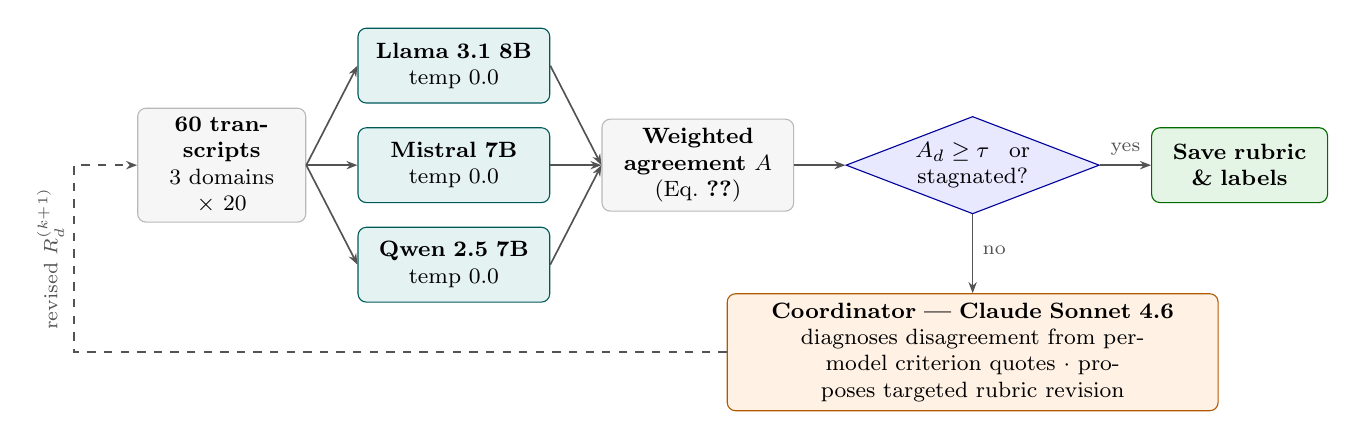
\begin{tikzpicture}[node distance=0.5cm and 0.65cm]
  \node[gbox=1.9cm] (corpus)
    {\textbf{60 transcripts}\\3 domains $\times$ 20};

  \node[pbox={teal}{2.2cm}, right=of corpus] (mistral)
    {\textbf{Mistral 7B}\\temp 0.0};
  \node[pbox={teal}{2.2cm}, above=0.3cm of mistral] (llama)
    {\textbf{Llama 3.1 8B}\\temp 0.0};
  \node[pbox={teal}{2.2cm}, below=0.3cm of mistral] (qwen)
    {\textbf{Qwen 2.5 7B}\\temp 0.0};

  \node[gbox=2.2cm, right=of mistral] (agree)
    {\textbf{Weighted agreement} $A$\\(Eq.~\ref{eq:agree})};

  \node[mydiamond, right=of agree] (dec)
    {$A_d \geq \tau$ \, or\\stagnated?};

  \node[pbox={green!60!black}{2.0cm}, right=of dec] (save)
    {\textbf{Save rubric}\\\textbf{\& labels}};

  \node[pbox={orange}{6.0cm}, below=1.0cm of dec] (coord)
    {\textbf{Coordinator --- Claude Sonnet 4.6}\\
     diagnoses disagreement from per-model criterion quotes $\cdot$
     proposes targeted rubric revision};

  \coordinate (fb) at ($(corpus.west)+(-0.8cm,0)$);

  \draw[arr] (corpus.east) -- (mistral.west);
  \draw[arr] (corpus.east) -- (llama.west);
  \draw[arr] (corpus.east) -- (qwen.west);
  \draw[arr] (llama.east)   -- (agree.west);
  \draw[arr] (mistral.east) -- (agree.west);
  \draw[arr] (qwen.east)    -- (agree.west);
  \draw[arr] (agree.east) -- (dec.west);
  \draw[arr] (dec.east) -- node[lbl,above]{yes} (save.west);
  \draw[arr] (dec.south) -- node[lbl,right,pos=0.45]{no} (coord.north);
  \draw[darr] (coord.west) -- (coord.west -| fb)
    -- node[lbl,rotate=90,anchor=south,midway]{revised $R_d^{(k+1)}$}
       (fb) -- (corpus.west);
\end{tikzpicture}}
\caption{CRUCIBLE system architecture. Three judge models evaluate
independently at temperature 0.0. The dashed arrow is the only feedback path:
a revised rubric flows back into the next iteration. No human input occurs
after initialization.}
\label{fig:arch}
\end{figure*}

\section{The CRUCIBLE System}

\subsection{Problem Statement}

Given a corpus $D = \{d_1,\dots,d_N\}$ to be annotated with a binary label
$y \in \{\mathrm{H},\mathrm{L}\}$, and an initial rubric $R^{(0)}$ specifying
criteria for each label, we seek a revised rubric $R^{(k)}$ such that the
weighted inter-judge agreement $A(R^{(k)}, D) \geq \tau$ for a target
threshold $\tau$, with the revision process requiring no human-labeled
reference data.

The key insight is that inter-judge disagreement encodes rubric
underspecification: when two competent models applying the same rubric reach
opposite conclusions on the same document, the rubric has not resolved the
case. A coordinator with visibility into both decisions and the
criterion-level justifications can identify which criterion was misapplied
and propose a targeted revision.

\subsection{Architecture}

Three local judge models (Llama 3.1 8B, Mistral 7B, Qwen 2.5 7B, each at
temperature 0.0) independently label every transcript against the current
domain rubric $R^{(k)}_d$, in isolation from one another. Their outputs feed
a weighted inter-judge agreement score $A$ (Eq.~\ref{eq:agree}); if a domain
is below threshold and has not stagnated, a coordinator (Claude Sonnet 4.6,
\citealp{anthropic2026sonnet46}) diagnoses the disagreement from per-model
criterion quotes, flags any irreducible cases, and proposes a targeted rubric
revision that feeds back into the next iteration. The loop stops when all
domains converge or after 10 iterations, emitting the calibrated rubrics,
labels, and a summary log. Figure~\ref{fig:arch} gives the full architecture.

\paragraph{Judge models.}
Three heterogeneous local models via Ollama at temperature 0.0, chosen to
represent different training lineages, maximizing the diagnostic value of
their disagreements. These serve as the calibration instrument only;
production labeling in the downstream application uses a separate, stronger
frontier ensemble \citep{das2026snr}.

\paragraph{Coordinator model.}
Claude Sonnet 4.6 \citep{anthropic2026sonnet46}, via API. Receives the
current rubric, per-model label assignments and criterion-level justification
quotes for each disagreement case, and disagreement counts per criterion;
produces a structured revision proposal specifying which criterion to modify.

\paragraph{Agreement metric.}
\begin{equation}
A = \frac{1}{N}\sum_{i=1}^{N} w_i,
\qquad
w_i = \frac{1}{K}\max_{c \in \mathcal{C}} n_{ic}
\label{eq:agree}
\end{equation}
where $K$ is the panel size, $\mathcal{C}$ the label set with $L = |\mathcal{C}|$,
and $n_{ic}$ the number of judges assigning label $c$ to item $i$; $w_i$ is the
panel's majority fraction on that item, and $A$ is bounded below by
$f_{K,L} = \lceil K/L \rceil / K$. This work uses $K = 3$ on a binary label,
where every item is either unanimous ($w = 1.0$) or a two--one majority
($w = 0.667$) and $f = 0.667$. Under independent judges the expected value of
$A$ is approximately $0.75$ at $K = 3$, the chance level for this metric; label
skew can raise it further. All-agree rate is tracked separately as a stricter
secondary metric.

\subsection{Calibration Loop}

Domain-specific rubrics $R^{(0)}_d$ are written at moderate abstraction. At
each iteration: all three judges evaluate all documents; weighted agreement
$A^{(k)}_d$ is computed per domain; for each non-converged, non-stagnated
domain below $\tau$, disagreement cases are extracted, per-model criterion
quotes assembled, and the coordinator proposes a revision applied to the next
iteration. A domain is marked stagnated when $\Delta A_d \leq 0$ for three
consecutive iterations and held at its current rubric; the loop terminates
only when all domains have converged or 10 iterations are reached. A
regression check re-evaluates each already-converged domain every iteration.

\subsection{Judge Quality Control}

Prior to the primary run, each candidate judge is screened for discriminative
validity. During development, Gemma 2 9B produced LOW labels for all 60
transcripts across all domains (0\% HIGH rate)---a degenerate judge providing
zero inter-judge signal. It was replaced with Qwen 2.5 7B before the
calibration run reported here. This pre-screening gate is itself a
risk-relevant safeguard: a degenerate judge inflates agreement without shared
understanding, and would silently pass an agreement-only quality check.
Separately, once a domain converges, CRUCIBLE re-evaluates it on each
subsequent iteration under the same rubric and judges as an output-stability
check; no regression (agreement drop $>10$ points) appeared in the reported
run.

\subsection{Columnar Evaluation Order}

Batching evaluation by model rather than by document (running each judge
across all 60 transcripts before switching models) reduces model-load events
from 180 to 3 per iteration and cuts per-iteration runtime from an incomplete
$>$30 minutes to 17--20 minutes on consumer hardware, making the full
10-iteration run tractable. This is an engineering detail, not a scientific
finding.

\section{Experimental Setup}
\label{sec:setup}

\paragraph{Task and corpus.}
Binary classification of YouTube educational video transcripts under the SNR
taxonomy: HIGH signal (substantive instructional content) vs.\ LOW signal
(generic motivational advice, fear-based framing, promotional material). The
corpus comprises 60 transcripts across three domains (20 per domain):
General Education, Technology \& AI, and Career \& Self-Improvement.

\paragraph{Sampling.}
Transcripts were collected via manual search ($\sim$20) and the YouTube Data
API v3 ($\sim$130, spanning this corpus and a 90-transcript held-out
supplement), prioritizing a fixed per-domain channel allow-list before
falling back to general search---a deliberate diversity-for-consistency
trade-off (Limitations).

\paragraph{Target threshold.}
$\tau = 0.80$: a modest margin above the metric's $\approx 0.75$ chance level
under independent judges, not a claim that $0.80$ represents strong
agreement. We treat $\tau$ as a practical stopping rule; chance-corrected
metrics (Fleiss' $\kappa$, \citealp{fleiss1971}; Gwet's AC1,
\citealp{gwet2008}) are what we rely on to judge genuine convergence.

\paragraph{Runtime.}
17--20 minutes per iteration, 170.7 minutes total; the run terminated at the
maximum-iteration cap of 10 on a consumer MacBook (Apple Silicon, no discrete
GPU).

\section{Results}
\label{sec:results}

\subsection{Per-Domain Convergence}

General Education converged immediately (iteration 1, no revision).
Technology \& AI required one revision: the coordinator diagnosed that Qwen
2.5 7B was reading the technical-specificity criterion too narrowly; the
revised criterion raised agreement from 76.7\% to 81.7\%, crossing threshold
in one step. Career \& Self-Improvement required two revision attempts: the
first (v1) reached 70.0\%, the second (v2) regressed to 68.4\% and was
discarded; agreement never approached the 80\% target
(Table~\ref{tab:trajectory}). The coordinator's diagnosis across both
iterations consistently identified the same failure mode: one judge applied
the ``generic motivational language'' criterion to any transcript containing
motivational phrasing, regardless of co-occurring procedural content.

\begin{table}[tb]
\centering
\caption{Calibration results per domain. $\kappa$ is Fleiss' $\kappa$
\citep{fleiss1971} and AC1 is Gwet's AC1 \citep{gwet2008}, both computed over
the three judges' labels.}
\label{tab:results}
\small
\begin{tabular}{lccc}
\toprule
\textbf{Domain} & \textbf{Best} $A$ & $\kappa$ & \textbf{AC1} \\
\midrule
General Education    & 96.7\% & $-0.034$ & $+0.929$ \\
Technology \& AI     & 81.7\% & $+0.246$ & $+0.286$ \\
Career \& S-I        & 70.0\% & $-0.350$ & $-0.080$ \\
\bottomrule
\end{tabular}
\end{table}

\begin{table}[tb]
\centering
\caption{Weighted agreement (\%) per domain across iterations. Career's
second revision (v2) regressed at iteration 3 and was not retained; the final
output is v1 (70.0\%, iteration 2). A check mark marks a domain at or above
$\tau = 0.80$.}
\label{tab:trajectory}
\small
\begin{tabular}{lccc}
\toprule
\textbf{Iter.} & \textbf{Career \& SI} & \textbf{Tech \& AI} &
\textbf{Gen.\ Edu.} \\
\midrule
1     & 68.4                 & 76.7            & 96.7 \checkmark \\
2     & 70.0                 & 81.7 \checkmark & 96.7 \checkmark \\
3     & 68.4 (regressed)     & 81.7 \checkmark & 96.7 \checkmark \\
4--10 & 68.4 (no further gain) & 81.7 \checkmark & 96.7 \checkmark \\
\bottomrule
\end{tabular}
\end{table}

We report Fleiss' $\kappa$ \citep{fleiss1971} and Gwet's AC1
\citep{gwet2008} alongside raw weighted agreement because raw agreement is
inflated by label prevalence (Table~\ref{tab:results}). Technology \& AI
shows fair chance-corrected agreement---the only domain where a rubric
revision carried agreement to the convergence target. Career \&
Self-Improvement shows below-chance agreement: the judges are systematically
anti-correlated relative to that metric's chance expectation, which no rubric
revision could change. General Education shows $\kappa \approx 0$ despite
96.7\% raw agreement---the known prevalence paradox of $\kappa$ under skewed
marginals \citep{byrt1993}, with Gwet's AC1 less affected
\citep{gwet2008}. The practical point: CRUCIBLE's contribution is not
raising raw agreement per se, but diagnosing which regime a domain occupies:
rubric-fixable, capability-bounded, or prevalence-dominated. Most of the final
agreement is accordingly attributable to the initial rubrics rather than to
revision: General Education converged with no revision at all, Technology \&
AI gained 5.0 points, and Career \& Self-Improvement gained 1.6 and never
approached $\tau$. This bounds any claim about the calibration loop's effectiveness as an agreement-raising mechanism, and is consistent with locating its value in diagnosis instead.

\paragraph{The stopping rule is satisfied before agreement is.}
Equation~\ref{eq:agree} assigns weight $0.667$ to every non-unanimous item, so
$A$ has a floor of $0.667$ when no item is unanimous. Solving
$A \geq \tau$ for the unanimous count $u$ over $N$ items gives
$u \geq (\tau - 0.667)\,N / 0.333$, which at $\tau = 0.80$ and $N = 20$ is
$u \geq 8$. The convergence criterion is therefore met when 40\% of items are
unanimous and 60\% still carry judge disagreement. Technology \& AI crossed $\tau$ with $u = 9$ of 20; General Education, which
converged without revision, had $u = 18$. The two outcomes the loop reports identically as ``converged'' differ by a
factor of two in unanimity and by $0.643$ in chance-corrected agreement
(AC1 $=0.286$ vs.\ $0.929$; Table~\ref{tab:results}). This is a property of
the threshold, not of the domains: any stopping rule on an agreement statistic
with a non-zero floor halts at a chance-corrected level fixed by that floor,
so $\tau$ must be set relative to the floor rather than on the unit interval
(the floor-normalised form is given below). We retain $A$ in the trajectory
tables because the loop optimized it, and report AC1 beside every value.

\paragraph{Pairwise structure of the panel.}
Panel-level $A$ also conceals which judges carry it. Llama~3.1~8B and
Mistral~7B are the highest-agreeing pair in every domain (100.0\%, 75.0\%,
90.0\%) and Qwen~2.5~7B is the systematic dissenter. Technology \& AI crossed
$\tau$ at the panel level while its Llama--Qwen pair agreed on only 45.0\% of
items, below that pair's own chance expectation (AC1 $=-0.08$): the crossing
is a two-of-three majority carried by the more HIGH-leaning pair, not a
uniform consensus---a second line of evidence, internal to the judges, that
the threshold is permissive. Career's non-convergence is near-total
anti-correlation rather than noise (Llama and Qwen agree on 2 of 20 items),
which no rubric revision reachable by this loop could repair, and the
prevalence effect recurs pairwise: General Education's Llama--Qwen pair scores
90.0\% raw agreement at Cohen's $\kappa = 0.00$.


\subsection{Human Validation}
\label{sec:humanval}

A known limitation of LLM-as-judge pipelines is that inter-judge agreement
among automated annotators may reflect shared model bias rather than
agreement with independent human judgment. We address this with an
independent human validation study covering the entire corpus: 20 transcripts
per domain, run in two rounds of 10. Each round recruited three annotators per
domain (18 annotators in total, Prolific approval rating above 95\%, recruited
via Prolific, \citealp{palan2018prolific}), and the two rounds drew disjoint
cohorts---no annotator appears in more than one round or more than one domain.
Round~1 scored the even-indexed transcripts of each domain block and round~2
the odd-indexed ones, a systematic rather than random split of the
60-transcript corpus. Annotators saw only the raw transcript
text---not the calibrated rubric, domain label, or CRUCIBLE's output---and
judged, with mandatory written justification, whether each transcript was
substantive or generic.

\begin{table}[tb]
\centering
\caption{Human validation at 20 transcripts per domain, scored by two disjoint
cohorts of three annotators (round~1 and round~2). AC1 is Gwet's AC1 among the three annotators
within a domain-round. Pooled over all 20 items, with 95\% percentile
bootstrap CIs (10{,}000 resamples over items), AC1 is $0.70$
$[0.43, 0.89]$ for General Education, $0.33$ $[-0.02, 0.64]$ for
Technology \& AI, and $0.24$ $[-0.06, 0.56]$ for Career \&
Self-Improvement.
``vs.\ CRUC.'' is the share of transcripts where human majority-vote consensus
matches CRUCIBLE's calibrated label. ``Base'' is the majority-class baseline:
the score a rater achieves by labelling every item with the domain's dominant
system-label class. Bold marks the only cell that exceeds its own baseline.}
\label{tab:humanval}
\footnotesize
\setlength{\tabcolsep}{3.5pt}
\begin{tabular}{@{}llccc@{}}
\toprule
\textbf{Domain} & \textbf{Rd} & \textbf{AC1} & \textbf{vs.\ CRUC.} &
\textbf{Base} \\
\midrule
Gen.\ Edu.      & 1 & $0.63$    & 90\%           & 100\% \\
                & 2 & $0.76$    & 100\%          & 100\% \\
Tech.\ \& AI    & 1 & $0.63$    & 50\%           & 60\%  \\
                & 2 & $-0.03$   & \textbf{80\%}  & 60\%  \\
Career \& S-I   & 1 & $0.33$    & 50\%           & 90\%  \\
                & 2 & $0.23$    & 80\%           & 90\%  \\
\midrule
\textbf{Overall} & & ---        & \textbf{75\%}  & 83\%  \\
\bottomrule
\end{tabular}
\end{table}

\begin{figure}[tb]
\centering
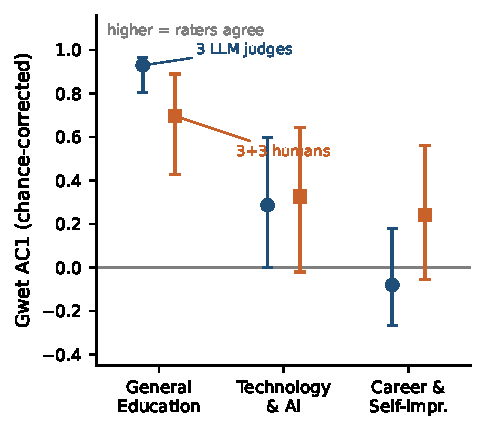
\includegraphics[width=\columnwidth]{fig_reliability.pdf}
\caption{Chance-corrected reliability for the three LLM judges and for the
human annotators, by domain. Both rater panels rank the domains identically
(Spearman $\rho = 1.00$ over three domains, descriptive only): the judges find
difficult what the humans find difficult. Bars are 95\% percentile bootstrap
intervals over items (10{,}000 resamples, $n = 20$ per domain per panel). The
two domains the calibration loop reports as converged sit at judge AC1
$=0.93$ and AC1 $=0.29$.}
\label{fig:humanval}
\end{figure}

Two results follow, and they point in different directions.

The first is a correspondence. Chance-corrected reliability among the human
annotators ranks the domains in exactly the order the judge panel does:
General Education highest (human AC1 $=0.70$ pooled, judge AC1 $=0.929$),
Technology \& AI second ($0.33$ vs.\ $0.286$), Career \& Self-Improvement
lowest ($0.24$ vs.\ $-0.080$). With three domains this is a rank statement
rather than a tested relationship, but the magnitudes agree closely in the two
harder domains, and the direction is unambiguous: the judges find difficult
what the humans find difficult. Figure~\ref{fig:humanval} (left) shows both rater panels with their
intervals. This correspondence is evidence against reading the judge panel's
failures as arbitrary, and it is the reason we relocate the paper's central
claim from human misalignment to the stopping rule.

The second is a negative result about the match statistic itself. Because each
domain's system labels are heavily skewed toward one class, a rater who assigns
that class to every item scores 100\%, 60\%, and 90\% in the three domains
respectively. Measured against that majority-class baseline, five of the six
domain-round cells in Table~\ref{tab:humanval} fail to beat a constant
labelling, and the pooled rate of 75\% is below the pooled baseline of 83\%.
The single exception is Technology \& AI round~2 (80\% against a 60\%
baseline). General Education's 100\% in round~2 ties a constant all-HIGH rater
exactly. We therefore report human--system match as uninformative in this
design and do not rest any claim on it.

\paragraph{What the enlarged sample does and does not establish.}
An earlier version of this study, at $n=10$ per domain, reported a
between-domain contrast in human--system match (9/10 vs.\ 5/10) as preliminary
evidence of an alignment dissociation, noting it did not reach significance on
its own (Fisher exact $p = 0.141$) and that roughly 19 items per domain would
be required for 80\% power. Doubling to $n=20$ did not confirm that contrast;
it removed its basis. Technology \& AI's match moved from 50\% to 80\% between
rounds, pooling to 65\%, and the majority-class correction above shows that
General Education's high match was never distinguishable from constant
labelling. We report this as a failed replication of our own earlier result.

On the reliability measures, where the enlarged sample does buy resolution, we
state what clears zero. Among the judges, General Education's AC1 exceeds
Technology \& AI's ($+0.64$, 95\% CI $[+0.31, +0.94]$) and Career's ($+1.01$,
$[+0.73, +1.21]$), and Technology \& AI over Career is marginal ($+0.37$, $[-0.01, +0.73]$). Among the humans, only General Education over Career clears
($+0.46$, $[+0.04, +0.80]$); General Education over Technology \& AI does
\emph{not} ($+0.37$, $[-0.04, +0.77]$) and Technology \& AI versus Career is
indistinguishable ($+0.09$, $[-0.39, +0.52]$). Technology \& AI's human AC1
does change between cohorts ($+0.66$, $[+0.03, +1.11]$), so its human
reliability is cohort-dependent where General Education's is not. At 20 items
and three raters per cohort these intervals are wide; we present the estimates
as a ranking with stated uncertainty, not as resolved effect sizes.

\paragraph{Scope of the reference set used by later analyses.}
The rubric-portability test, the reasoning-before-label ablation and the
frontier-ensemble comparison below all score against the original round-1
30-item reference and were not re-run at $n=20$. Their numbers are correct for
what they measure, but they inherit the limitation above---human-consensus
match is a weak statistic in this design---so they are evidence about
consistency across system configurations, not about human alignment.

Automated convergence correctly identified General Education's annotator group
as reliable and Career \& Self-Improvement's as difficult, and the human data
now confirm that ordering directly. What it did not do is signal that
Technology \& AI's crossing of $\tau$ rested on 9 unanimous items out of 20.
That is the paper's risk-assessment finding in its corrected form: the failure
is in the stopping criterion, not in the judges' relationship to human
judgment. An operator needs the chance-corrected value and the floor of the
metric being thresholded, not the thresholded value alone. We did not
recalibrate rubrics toward the human labels, to avoid reintroducing
circularity; the study's role is diagnostic, not corrective.

\subsection{Judge Replacement}

Replacing the diagnosed bottleneck judge with a different model on Career
raised inter-judge agreement ($0.700 \rightarrow 0.883$), but the
majority-vote label changed on 0 of the 20 transcripts: the two retained
judges already agreed 90\% of the time, so no third judge could change the
output. This is a unanimity effect (2--1 becoming 3--0), not an actual
annotation change---a cautionary result for any risk assessment that treats
rising agreement as evidence of improving accuracy without checking whether
the underlying labels moved at all. This finding is consistent with, but does
not independently establish, the paper's central claim, given a structural
confound in the panel tested here (the two retained judges' pre-existing
90\% agreement).

\subsection{Rubric Portability Across Judge Models}
\label{sec:portability}

A natural question is why a single frontier model, applied zero-shot, would
not suffice in place of the full calibration loop. We test this
directly, and in doing so obtain the first of two probes of whether movement
in the optimized metric tracks movement in agreement with the human
reference. Both probes share that reference, so they test robustness to the
judge model and to prompt structure rather than supplying independent
evidence.

We compare three approaches against the same 30-transcript human reference
used above: (1)~the local three-judge panel applying its calibrated rubric;
(2)~GPT-5.6~Sol \citep{openai2026gpt56sol} applying a naive zero-shot prompt
with no rubric; and (3)~GPT-5.6~Sol applying the same calibrated rubric used
by the local panel. We use a non-Anthropic model for this baseline because
Claude serves exclusively as the calibration coordinator throughout this work
and was not evaluated as a judge, to avoid conflating baseline performance
with the model family responsible for rubric design. GPT-5.6~Sol does not
support temperature\,$=$\,0 at time of writing; results reflect the model's
default sampling temperature.

Against the round-1 human reference ($n=30$, 10 per domain), the local
calibrated panel and a single zero-shot frontier pass achieve identical
aggregate accuracy (both 63.3\%; per domain 50/50/90\% for the local panel
and 60/30/100\% for GPT-5.6~Sol on Career, Technology \& AI and General
Education), so the 10-iteration loop does not categorically outperform one
frontier zero-shot pass. Giving the frontier model the \emph{same} calibrated
rubric does not add value and drops it to 50.0\% overall, degrading Career
substantially (60\% $\rightarrow$ 20\%). Comparing the same
frontier model's outputs against the local panel's labels directly, rather
than against human judgment, shows the rubric \emph{does} make GPT-5.6~Sol's
outputs converge toward the local panel's specific behaviour (agreement with
the local panel rises from $0.500$ to $0.633$ when the rubric is added).
Taken together, the calibrated rubric teaches a frontier judge to mimic the
local ensemble's particular behaviour pattern---including the local
ensemble's specific errors---rather than making it more accurate against the
human reference. The comparison is within-intervention---the same items scored with and without
the rubric---so unlike the between-domain contrast in the
Human Validation section it does not rest on per-domain sample size, but it
inherits that section's finding that human-consensus match is
prevalence-dominated here. We therefore read it as evidence about what the
rubric transfers (the panel's behaviour, including its errors), not as a
measurement of alignment. It is not a single-draw artifact: repeating both
variants five times per transcript (600 calls) gives 87--93\% of transcripts
an identical label across all five draws, with majority-of-five accuracy
matching the single-draw result exactly.

For deployment this means a rubric calibrated against one judge panel should
not be assumed portable without re-validation, and rising agreement after
transfer is specifically not evidence that the transfer succeeded.

\subsection{Reasoning-Before-Label Ablation}
\label{sec:cot}

Motivated by the question of whether Career \& Self-Improvement's stagnation
reflects a single-pass prompting limitation rather than a true capability
ceiling, we added an intermediate reasoning step to the local judges'
prompts, in the style of chain-of-thought prompting
\citep{wei2022chainofthought} (reasoning generated before the label, not
after), and re-scored all three domains against their existing calibrated
rubrics using the same three local models at temperature\,$=$\,0.0. We call
this a \emph{reasoning-before-label prompt} rather than chain-of-thought
throughout, since we have no access to the models' actual internal
computation---only to text generated before the label in response to an
instruction to reason first.

The reasoning step reliably raises inter-judge agreement in the two domains
with room to improve---Career $A$ $0.684 \rightarrow 0.767$ ($+8.3$ points)
and Technology \& AI $0.817 \rightarrow 0.933$ ($+11.6$ points, with AC1
nearly tripling)---but it never \emph{helps}, and in Career actively
\emph{hurts}, agreement with the human reference: Career falls
$50\% \rightarrow 40\%$ (Cohen's $\kappa$, \citealp{cohen1960}, flips $+0.14
\rightarrow -0.25$), Technology \& AI is flat at $50\%$ while its AC1 drops,
and General Education is unchanged at $90\%$ while dipping slightly on
inter-judge agreement ($0.967 \rightarrow 0.917$), consistent with a ceiling
effect.

This rules out simple single-pass prompting failure as the sole explanation
for Career \& Self-Improvement's stagnation---the judges \emph{can} be made
to agree more with reasoning added---but shows that forcing
reasoning-before-label makes the panel more internally consistent without
making that consistency more correct. It is the second probe of whether the optimized
metric tracks anything beyond itself: a $+11.6$-point movement in $A$ leaves
agreement with the human reference flat. Like the portability test it scores
against the same 30 human labels and inherits their prevalence limitation, so
it does not enlarge the evidence base; what it establishes is that $A$ can be
moved substantially by a prompt change alone, which is a further reason not to
read a threshold crossing on $A$ as evidence of improved annotation. We revise our diagnosis of Career accordingly. The enlarged human study shows that Career's human annotators
agree with each other barely above chance themselves (AC1 $=0.24$ pooled,
95\% CI $[-0.06, 0.56]$), the lowest of the three domains and matching the
judges' own ordering. The stagnation is therefore better read not as judges
failing to reach a well-defined human standard, but as a domain in which the
substantive/generic distinction is weakly determined for judges and humans
alike---the capability-bounded cell of our trichotomy, now with rater-side
evidence. Explicit reasoning raises internal consistency without supplying
the missing construct. We used
a single, untuned reasoning-before-label prompt design across all domains;
whether a more carefully engineered prompt would alter this pattern is
untested.

\subsection{Additional Diagnostic Analyses}

Four further diagnostic analyses are summarized here, with full designs in
the companion technical report \citep{das2026snr}.

\paragraph{Held-out generalization.}
Re-scoring calibrated rubrics on a 90-transcript unseen set improves the
weighted inter-judge agreement metric for Career \& Self-Improvement
(72.3\% $\rightarrow$ 78.9\%) and Technology \& AI
(84.5\% $\rightarrow$ 87.8\%), though the majority-vote annotation changes on
0 of the 90 transcripts---only the metric moves, not any output label.
``Held-out'' here means document-held-out, not source-held-out: the 60- and
90-transcript corpora share 6 of 46 and 50 channels respectively. The held-out
corpus is also 100\% majority-vote HIGH in every domain, so this result shows
that unambiguous HIGH labels are stable under the calibrated rubric---not that
HIGH/LOW discrimination generalizes.

\paragraph{Downstream classifier case study.}
As a usability case study, not a validation of agreement with the human
reference, an SVM trained on calibrated-rubric labels achieved
$F_1 = 0.871$ (recall $= 0.964$) on HIGH-signal, vs.\ $F_1 = 0.000$ for a
majority-class baseline \citep{das2026snr}. That study uses the companion
report's separate corpus---89 real transcripts labeled by a frontier ensemble
plus 300 synthetic transcripts added for class balance---so its class
distribution is not that of the 60-transcript corpus above.

\paragraph{Frontier ensemble vs.\ human judgment.}
The separate frontier ensemble that produced the classifier's training labels
tracks human judgment about as loosely as the local panel (56.7\% vs.\
63.3\%; a full-3-judge-subset check gives a consistent 55.0\%), so the classifier's $F_1 = 0.871$ rests on similarly-reliable labels. Both
figures are measured against the round-1 reference and inherit its prevalence
limitation, so we report them as showing that a stronger,
separately-configured ensemble behaves no differently here---not as a
measurement of alignment.

\paragraph{Irreducible cases.}
The coordinator flagged two Technology \& AI transcripts as irreducible
(genuine ambiguity, not rubric failure) and excluded them from stagnation
counting. For this domain, the convergence conclusion (81.7\%, above
threshold) is identical whether these cases are included or excluded from the
denominator. Re-auditing which two transcripts were flagged proved infeasible: the
pipeline persists only calibrated rubrics, labels and a run summary, and
flagged indices are held in memory only. As an upper bound, 11 of 20
Technology \& AI transcripts still show inter-judge disagreement under a full
final-rubric relabel---a superset of the two, not those specific cases.

\paragraph{Panel size.} Eq.~\ref{eq:agree} holds for arbitrary $K$ and $L$, but a
fixed $\tau$ does not transfer across panel sizes, because $f_{K,L}$ is
non-monotonic in $K$: for a binary label it is $0.500$, $0.667$, $0.500$ and
$0.600$ at $K = 2,3,4,5$, since even panels admit ties. A fixed $\tau = 0.80$
therefore sits $0.60$, $0.40$, $0.60$ and $0.50$ of the way from floor to ceiling
at those sizes---the $K = 3$ panel used here is the most permissive of any small
panel, not the strictest---and cross-$K$ comparison requires the floor-normalised
$A^{*} = (A - f_{K,L})/(1 - f_{K,L})$. The judge-replacement diagnostic tests this directly. Across all subsets of
the four judges scored on Career \& Self-Improvement, raw $A$ ranks the
three-judge Llama--Mistral--Granite panel ($88.3\%$) above the two-judge
Mistral--Granite panel ($87.5\%$) while $A^{*}$ reverses them ($65.0\%$
vs.\ $75.0\%$), with two further inversions. Raw $A$ is therefore
interpretable only at fixed $K$, and $\tau$ must be re-derived per panel size.
This is demonstrated in one domain at $K \le 4$; the generalisation itself is
exact by construction.


\subsection{Robustness of the Human Validation Result}
\label{sec:robustness}

Two checks probe the stability of the round-1 human study. Both were computed
on that round's 30 items and were not re-run after the sample was enlarged;
they are retained because they bear on the annotator-rejection decision and on
channel clustering, neither of which the enlarged sample addresses.

\paragraph{Annotator-rejection sensitivity.}
One of nine Prolific submissions (Technology \& AI) was rejected on a
multi-factor judgment (completion time, an attention-check failure, low-effort
justifications) and replaced. Recomputing this domain's human consensus with
the rejected annotator's original responses reinstated in place of the
replacement changes zero of the 10 item-level consensus labels.
Local-panel-vs-human agreement for Technology \& AI is identical under both
the official and reinstated consensus (50.0\%, Cohen's $\kappa = -0.19$,
Gwet's AC1 $= 0.20$), so this domain's reported divergence does not depend on
the rejection decision.

\paragraph{Channel-clustering sensitivity.}
Resampling at the channel level rather than the transcript level (10{,}000
resamples, 27 unique channels of 30 items) shifts the round-1 intervals only
modestly---the overall upper bound moves 80.0\% to 79.3\%---so clustering has
a small effect on that sample. Source-channel metadata is not retained per
transcript in the released corpus file, so the check could not be extended to
all 60 items; clustering at that scale (up to 5 transcripts per channel)
remains unquantified.

\subsection{Reproducibility of the Original Run}

We recovered the run timestamp, current model digests, quantization
(Q4\_K\_M for all three judges) and context windows via \texttt{ollama show},
and confirmed from the judge-calling code that temperature was explicitly 0.0
with no context-window override, ruling out truncation as an explanation for
the observed misreadings. We could not recover shell history for the original
model pulls, coordinator API logs, or a digest snapshot to diff against, so
the follow-up analyses were run under the closest recoverable configuration
and should be read as diagnostic extensions rather than exact controlled
replications.

\section{Discussion}

The Career \& Self-Improvement ceiling shows a class of disagreement that
rubric revision did not fix under this judge and prompt setup. An operator
seeing 70.0\% agreement would not know whether to keep revising the rubric or
replace the judge; the stagnation pattern and the coordinator's consistent
diagnosis suggest the rubric was not the limiting factor, though judge
replacement could not fully separate this from a structural property of the
panel.

For AI risk assessment specifically, the paper's contribution is narrower and
more actionable than we first claimed. It is not that automated judges
systematically diverge from human judgment---the enlarged human study gives no
support for that, and the reliability
correspondence reported above argues against it. It is that a convergence
criterion defined on an uncorrected agreement statistic reports success at a
level of actual agreement determined by that statistic's floor. An operator
who reads 81.7\% as ``converged'' is reading a number that cannot fall below
66.7\% and that corresponds here to a chance-corrected AC1 of $0.286$. The
deployment risk is not a confidently-wrong evaluator; it is a stopping rule
that halts while most items are still contested, and a reported figure that
conceals this by construction. The remedy is arithmetic rather than
procedural: threshold a chance-corrected statistic, or set $\tau$ relative to
the floor of the statistic being used.

More broadly, agreement-based confidence bounds (Eq.~\ref{eq:agree}) are
informative only conditional on both the panel's construct validity and the
scale of the statistic being thresholded. CRUCIBLE's three-way
split---rubric-fixable, capability-bounded, prevalence-dominated---offers a
reusable vocabulary for characterizing residual disagreement, and this paper
supplies an instance of the third category applying to a paper's own headline
measurement: the human--system match rates we previously reported as evidence
are prevalence-dominated, and we retract them as such.

\section{Limitations}

\begin{itemize}
\item \textbf{Single experiment.} 60 transcripts, three domains;
      generalization to other domains or document types is untested.
\item \textbf{Statistical resolution of the human study.} The human study now
      covers the full corpus at $n=20$ per domain, which is the sample size an
      earlier version of this work identified as required. It did not resolve
      the comparison it was intended to resolve: the human--system match
      contrast disappeared under the majority-class correction, and on the
      reliability measures General Education over Technology \& AI still does
      not clear zero ($+0.37$, $[-0.04, +0.77]$). Three raters per cohort is
      the binding constraint, not the item count; resolving the human-side
      domain ordering would require more raters per item rather than more
      items.
\item \textbf{Non-standard agreement metric.} The calibration loop optimizes
      $A$ (Eq.~\ref{eq:agree}), whose $0.667$ floor is the subject of this
      paper's central finding. We report AC1 alongside it throughout, but the
      calibration trajectories, the stopping decisions, and therefore the
      released rubrics are all products of the uncorrected statistic. A
      re-run thresholding AC1 directly would likely produce different
      rubrics and different per-domain outcomes; we have not performed it.
\item \textbf{Two-cohort pooling.} The 20 items per domain were scored by two
      disjoint cohorts of three. Pooled AC1 therefore mixes within-cohort and
      between-cohort variation, and we report per-round values alongside every
      pooled figure for this reason. Technology \& AI's cohort-dependent
      reliability shows the mixing is not negligible.
\item \textbf{Model-specific ceiling.} The Career ceiling is diagnosed for one
      judge model (Qwen 2.5 7B) under one untuned prompt template; the
      reasoning ablation only partially addresses prompt reformulation, so the
      ceiling should not be called inherent to the model.
\item \textbf{Human-validation design.} Unaided judgment only; a
      rubric-guided condition would additionally test whether humans agree
      with the rubric's operational criteria rather than with intuition. Each
      domain also drew a distinct annotator set, so domain and cohort effects
      cannot be fully separated.
\item \textbf{Coordinator dependency and run reproducibility.} A
      non-bit-reproducible frontier coordinator gives an estimated $\pm 1$--2
      point run-to-run variance (unverified, single run); Career's iteration-2
      gain falls within that band. Model digests, quantization and context
      window were recovered from available logs and are consistent with, but
      not proof of, the original configuration; coordinator API logs were not
      accessible.
\item \textbf{Baselines and judge replacement.} No baseline beyond a single
      frontier judge was run against manual rubric revision or coordinator-free
      self-refinement, and judge replacement was tested once on a domain where
      the two retained judges already agreed 90\% of the time.

\end{itemize}

\section{Ethics Statement}

Human validation used Prolific \citep{palan2018prolific}. No formal
institutional ethics review or exemption was sought; participation followed
Prolific's standard consent, compensation exceeded the platform minimum, and only
pseudonymous IDs were collected.

\section{Conclusion}

CRUCIBLE demonstrates that annotation rubric calibration can be automated
through a coordinator-mediated iterative loop driven by inter-judge
agreement, with no human reference labels used during optimization. This
paper's central finding, however, concerns the criterion that decides when the
loop has succeeded. Because the weighted agreement statistic the loop optimizes
has a floor of $0.667$, a threshold of $\tau = 0.80$ is satisfied at 40\%
unanimity, and the domain that crossed it did so with a chance-corrected
agreement of $0.286$. A human validation study spanning the full corpus, at double the sample size
of our earlier report, does not support the human-alignment dissociation we
previously described as preliminary: judge and human reliability rank the
three domains identically, and match against human consensus fails to beat
majority-class labelling in five of six cells. For trustworthy AI evaluation,
the actionable takeaway is that a stopping rule must be defined on a statistic
whose scale is known---an automated judge panel reporting agreement above a
threshold is making a claim only as strong as the floor of the metric
thresholded.

\section{Code and Data Availability}
Code, data, rubrics, consolidated human ratings (60 transcripts, both
cohorts) and the reproduction script:
\url{https://github.com/biditdas18/rubric-calibration-agent}.

\bibliography{references}

\end{document}
